\section{Лабораторная работа 4 (Вариант 4)}
\subsection{Задание}

Выполнить классификацию двухмерных данных при помощи сети с самоорганизацией на основе конкуренции, обучающейся по алгоритму нейронного газа.

\subsection{Описание сетей с самоорганизацией на основе конкуренции}
Сетями с самоорганизацией называются сети, не требующие для своего
обучения «учителя» и самостоятельно адаптирующие свои веса под обучающие
данные. Такие сети строятся из нейронов типа WTA и подобных
им. Как правило, это однослойные сети, в которых каждый нейрон получает
все компоненты входного вектора $X$ размерностью $N$. На рисунке \ref{img:schemeNet_lab3}
представлена структурная схема такой сети.

\begin{figure}[H]
\centering
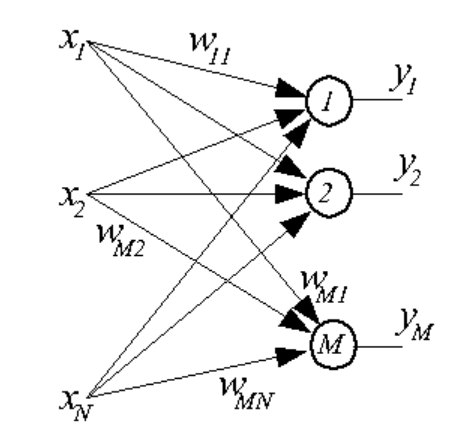
\includegraphics[scale=0.5]{schemeNet_lab3.png}
\caption{Схема сети с самоорганизацией на основе конкуренции}
\label{img:schemeNet_lab3}
\end{figure}

Веса входных связей $i$-ого нейрона образуют вектор
\begin{equation}
    W_{i} = \left[ \begin{array} { l l l l }{w_{i 1}} & {w_{i 2}}&{\dots}&{w_{ i N }}\end{array}\right]^{T} .
\end{equation}

Кроме связей, явно представленных в схеме, на этапе обучения имеют место
связи между нейронами, позволяющие судить о степени «соседства»
нейронов друг с другом, при этом смысл понятия «соседство» может
быть разным.
Укрупненно процесс обучения сети выглядит следующим образом. На
вход сети подается обучающий вектор $X^k$, для каждого нейрона определяется
$d(X^k, W_i)$ — расстояние (в смысле выбранной метрики) между
векторами $X_k$ и $W_i$. Определяется нейрон–победитель, для которого это
расстояние оказывается наименьшим. Вокруг нейрона–победителя образуется окрестность $S^k_w$ из нейронов–соседей с известным «расстоянием» до победителя. Веса нейрона–победителя и веса его соседей из $S^k_w$ уточняются, например, по правилу Кохонена:

\begin{equation}
	W_{i}^{k+1} = W_{i}^{k}+\eta_{i}^{k}\left(X^{k}-W_{i}^{k}\right) ,
\end{equation}

где $\eta^k_i$ --- коэффициент обучения, значение которого уменьшается с увеличением расстояния от $i$-ого нейрона до победителя. Веса нейронов вне $S^k_w$ не изменяются. Размер окрестности $S^k_w$ и величина $\eta^k_i$ с течением времени обучения уменьшаются.

В качестве меры измерения расстояния между векторами чаще всего
используются:

\begin{itemize}
\item евклидова мера $d \left( X , W _ { i } \right) = \left\| X - W _ { i } \right\| = \sqrt { \sum _ { j = 1 } ^ { N } \left( x _ { j } - w _ { i j } \right) ^ { 2 } }$
\item скалярное произведение
$d \left( X , W _ { i } \right) = 1 - X \cdot W _ { i } = 1 - \| X \| _ { 2 } \cdot \left\| W _ { i } \right\| _ { 2 } \cdot \cos \left( \angle X W _ { i } \right)$

\item манхэттеновское расстояние $d \left( X , W _ { i } \right) = \sum _ { j = 1 } ^ { N } \left| x _ { j } - w _ { i j } \right|$;

\item m-норма $d \left( X , W _ { i } \right) = \max _ { j } \left| x _ { j } - w _ { i j } \right|$.
\end{itemize}

\subsection{Проблема мертвых нейронов}
\label{seq:deadNeurons}
При «слепом» (как правило, случайном) выборе начальных значений весов
часть нейронов может оказаться в области пространства, в которой
отсутствуют обучающие данные или где их количество ничтожно мало.
Такие нейроны имеют очень мало шансов на победу в конкурентной
борьбе и адаптацию своих весов, вследствие чего они остаются мертвыми.
В итоге уменьшается количество активных нейронов, участвующих
в анализе входных данных, и, следовательно, увеличивается погрешность
их интерпретации, называемая погрешностью квантования. Встает проблема
активации всех нейронов сети на этапе обучения.
Такую активацию можно осуществить, базируясь на учете количества
побед, одержанных каждым нейроном в ходе обучения. Существуют
разные механизмы такого учета.
В одном из таких подходов каждому нейрону сети приписывается
потенциал $\pi_i$
, значение которого модифицируется после предъявления
каждого обучающего вектора $X^k$ по следующей формуле (в ней $w$ —
индекс нейрона-победителя):

\begin{equation}\label{eq:system}
		\begin{aligned}
		&	\pi _ { i } ^ { k + 1 } = \pi _ { i } ^ { k } + 1 / M, где i \neq w\\
		&   \pi _ { i } ^ { k + 1 } = \pi _ { i } ^ { k } - \pi _ { min }, где i = w.
		\end{aligned}  		
\end{equation}

где $\pi_{min}$ — минимальный потенциал, разрешающий участие в конкурентной борьбе. Максимальное значение потенциала устанавливается равным 1. На практике хорошие результаты получены для $\pi_{min} = 0.75$ .

\subsection{Алгоритм обучения}

Целью обучения сети с самоорганизацией на основе конкуренции является минимизация погрешности квантования:

\begin{equation}
 E _ { q } = \frac { 1 } { p } \sum _ { k = 1 } ^ { p } d \left( X ^ { k } , W _ { w ( k ) } \right)
\end{equation}

где $p$ — количество обучающих векторов $X^k$, $W_{w(k)}$ — вектор весов нейрона–победителя при предъявлении вектора $X^k$.
Примеры результатов обучения, близких к оптимальным, представлены
ниже на рисунках. Используются сети с 15 и 22 нейронами и двухкомпонентным входным вектором $X = \left[ x _ { 1 } , x _ { 2 } \right] ^ { T }$. На левых картинках (рисунок \ref{img:somNetr}) представлено распределение данных в обучающих выборках, на правых --- распределение весов нейронов обученной сети.

\begin{figure}[H]
\centering
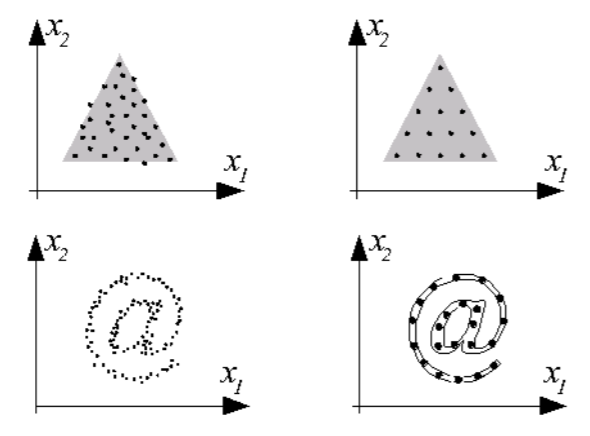
\includegraphics[scale=0.5]{somNet.png}
\caption{Схема сети с самоорганизацией на основе конкуренции}
\label{img:somNetr}
\end{figure}



\subsection{Алгоритм Кохонена}

В нейронных сетях, предложенных Т. Кохоненом (1982 г.), соседство нейронов
носит чисто топологический характер. В простом случае нейроны
слоя Кохонена образуют одномерную цепочку, при этом каждый нейрон
имеет, в общем случае, двух ближайших соседей (слева и справа).
В более сложном случае нейроны Кохонена образуют двумерную сетку
с четырьмя соседями у каждого нейрона (слева, справа, сверху, снизу).
В еще более сложном случае сетка гексагональна — у каждого нейрона
шесть соседей на плоскости (по циферблату часов — 2, 4, 6, 8, 10, 12
часов).
Коррекция весов нейронов в ходе обучения выполняется по формуле

\begin{equation}
W _ { i } ^ { k + 1 } = W _ { i } ^ { k } + \eta ^ { k } G ^ { k } \left( i , X ^ { k } \right) \left( X ^ { k } - W _ { i } ^ { k } \right),
\end{equation}


где функция соседства $G ^ { k } \left( i , X ^ { k } \right)$ определяется, как правило, формулой Гаусса в вид

\begin{equation}
G ^ { k } \left( i , X ^ { k } \right) = \exp \left( - \frac { d ^ { 2 } \left( i , X ^ { k } \right) } { 2 \left( \sigma ^ { k } \right) ^ { 2 } } \right),
\end{equation}

где $d \left( i , X ^ { k } \right)$ ---  расстояние от $i$-ого нейрона до нейрона–победителя с индексом $w_k$ в $k$-ом цикле обучения. При этом $d \left( w ^ { k } , X ^ { k } \right) = 0 , d \left( i , X ^ { k } \right) = 1$ для всех ближайших соседей $w_k$, $d(i, X^k) = 2$ для всех «внешних» ближайших соседей ближайших соседей нейрона победителя с индексом $w^k$ и так далее.

Как обычно, коэффициент обучения $\eta^k$ и параметр ширины функции
Гаусса $\sigma^k$ уменьшаются в ходе обучения (с ростом $k$). В результате обучения слоя Кохонена по такому алгоритму топологически
соседние нейроны становятся типичными представителями кластеров обучающих данных, соседствующих в многомерном пространстве.
В этом достоинство сетей Кохонена, называемых также картами Кохонена, — наглядность в представлении (путем одномерной или двумерной
визуализации) многомерных данных.

Очевидным практическим приложением сетей с самоорганизацией является
сжатие (с потерями) данных, в частности, покадровое сжатие изображений.
Но мы воспользуемся ей для других целей.
Важным свойством сетей с самоорганизацией на основе конкуренции
является способность к кластеризации данных и их распознаванию. Это
обеспечивает их широкое применение для решения задач диагностики,
например, неисправностей оборудовани


\subsection{Алгоритм нейронного газа}
В алгоритме нейронного газа адаптация весов происходит по формуле:
\begin{equation}\label{equ:weightCalc}
    W _ { i } ^ { k + 1 } = W _ { i } ^ { k } + \eta ^ { k } G ^ { k } \left( i , X ^ { k } \right) \left( X ^ { k } - W _ { i } ^ { k } \right),
\end{equation}
В каждом цикле обучения все нейроны сортируются в последовательности возрастания расстояния $d(w^k, X^k)$
\begin{equation}\label{equ:compareLenght}
    d _ { 0 } < d _ { 1 } < \ldots < d _ { j } < \ldots < d _ { M - 1 },
\end{equation}
где $j=m(i)$ — номер i-ого нейрона в последовательности. Для нейрона-победителя $m(i)=0$.

Значение функции соседства i-ого нейрона $G^k(i,X^k)$ определяется следующим выражением:
\begin{equation}\label{equ:neightbourFunc}
G ^ { k } \left( i , \mathbf { X } ^ { k } \right) = \exp \left( - \frac { m ( i ) } { \sigma ^ { k } } \right),
\end{equation}
где $\sigma ^k$ определяет уровень соседства и является величиной, уменьшающейся по ходу обучения. При $\sigma ^k$, стремящемся к 0, алгоритм превращается в алгоритм WTA. Для достижения хороших результатов самоорганизации сети обучение должно начинаться с большого значения $\sigma ^k$, которое с течением времени обучения уменьшается до 0. Для такого уменьшения $\sigma ^k$ предлагается использовать выражение:
\begin{equation}\label{equ:sigma}
    \sigma ^ { k } = \sigma ^ { \max } \cdot \left( \frac { \sigma ^ { \min } } { \sigma ^ { \max } } \right) ^ { \frac { k } { k _ { \max } } },
\end{equation}
где $k_max$ — максимальное заданное количество циклов обучения.

Коэффициент обучения $\eta_i^k$ тоже может уменьшаться с течением времени обучения, это уменьшение может быть линейным от $\eta_max$ в первом цикле до $\eta_min$ в цикле $k_max$, так и показательно в соответствии с формулой:
\begin{equation}\label{equ:eta}
    \eta ^ { k } = \eta _ { \max } \cdot \left( \frac { \eta _ { \max } } { \eta \max } \right) ^ { \frac { k } { k _ { \max } } }.
\end{equation}


\subsection{Реализация}

При поступлении очередной порции данных на вход нейронной сети в рамках каждой эпохи обучения, просходит подсчет весов по формуле \ref{equ:weightCalc}. Но перед этим необходимо определит евклидово расстояние между значениями вектора весов и значениями вектора входных значений, а так же величину функции соседства. В отличие от алгоритма Кохенена, где соседство нейронов определяется близостью их порядкового номера относительно победителя, в алгоритме нейронного газа соседство определяется величиной расстояния до победителя. То есть необходимо для каждого нейрона сначала посчитать расстояние до входных значений по формуле \ref{equ:euclid}, а затем отсортировать в порядке увеличенич значения расстояния (\ref{equ:compareLenght}). Таким образом, первый элемент $d(0)$ в отсортированном массиве расстояний - победитель. Далее нам надо получить индекс нейрона, которому принадлежит это значение расстояния. При расчете функции соседсва для i-го нейрона по формуле \ref{equ:neightbourFunc} мы используем этот индекс нейрона-победителя. Таким образом, нейрон, расположившийся ближе к победителю, значительнее откорректирует свои веса, что нельзя сказать про самый последний, дальний нейрон.

\begin{equation}\label{equ:euclid}
    d \left( X , W _ { i } \right) = \left\| X - W _ { i } \right\| = \sqrt { \sum _ { j = 1 } ^ { N } \left( x _ { j } - w _ { i j } \right) ^ { 2 } }
\end{equation}

Стоит сказать о двух параметрах:
\begin{itemize}
    \item Коэффециент обучения $\eta^k$, где k - номер цикла обучения
    \item Коэффециент соседства $\sigma^k$, где k - номер цикла обучения
\end{itemize}

По мере увеличения времени(итераций), значения коэффициентов $\eta ^ { k }$ и $\sigma ^ { k }$ должны уменьшаться. Для их расчета используются формулы \ref{equ:eta} и \ref{equ:sigma} соответсвенно. Изменяя значение параметра $\eta_{min}$ мы меняем скорость уменьшения коэффециента обучения, $\eta = 0 ... 1$. Величина $\sigma$ может принимать произвольные значения.


Проблема мертвых нейронов на начальном этапе обучения решается путем введения потенциалов (см. раздел \ref{seq:deadNeurons}). 
Минимальный потенциал принимается равным $\pi_{min} = 0.75$ и присваивается изначально всем нейронам.



\subsection{Обучение}
Выборка, на которой происходит обучение, и первоначальное расположение 16-ти нейронов показаны на рис. \ref{img:startpos}.

\begin{figure}[H]
\centering
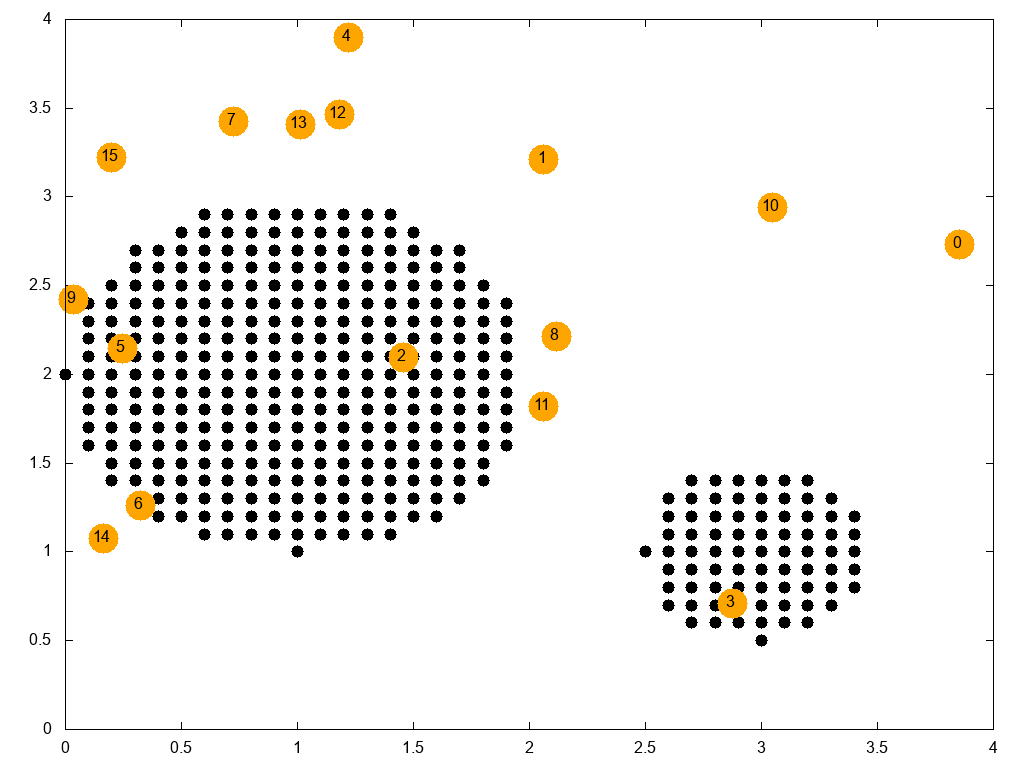
\includegraphics[scale=0.4]{netstartpos.png}
\caption{Обучающая выборка и расположение весов при инициализации}
\label{img:startpos}
\end{figure}

Веса разыграны по равномерному распределению вдоль каждой координатной оси в диапазоне от 0 до 4.

Для того, чтобы дать каждому нейрону возможность проявить себя и ликвидировать мертвые нейроны, произведено $M = 32$ итерации предварительного обучения. При этом использовались слудующие значения коэффециентов:

Значения параметров:
\begin{equation}
	\begin{aligned}
	 &	\sigma_{min} = 0.5,  \\ 
	 &	\sigma_{max} = 2.1, \\	
	 &	\eta_{min} = 0.5,  \\ 
	 &	\eta_{max} = 1, \\
	\end{aligned}
\end{equation} 

В результате, нейроны расположились следующим образом:

\begin{figure}[H]
\centering
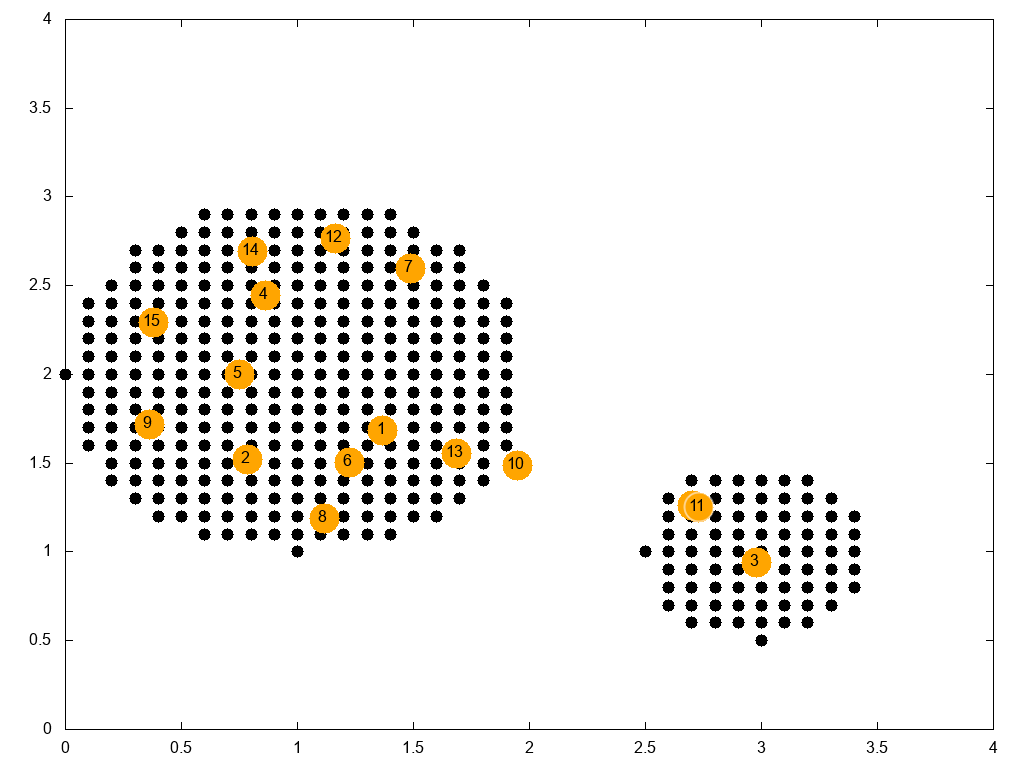
\includegraphics[scale=0.4]{netafterPreTrain.png}
\caption{Расположение нейронов после предварительного обучения ("оживления")}
\label{img:afterPreTrain}
\end{figure}

Для полноценного обучения, при котором больше не происходит изменения потенциалов нейронов, произведен обход входных данных в 10 эпох. Завершение работы алгоритма происходит при окончании всех эпох обучения, без учета минимизации величины ошибки квантования.
Параметры при этом заданы следующие:

\begin{equation}
	\begin{aligned}
	 &	\sigma_{min} = 0.01,  \\ 
	 &	\sigma_{max} = 1., \\	
	 &	\eta_{min} = 0.001,  \\ 
	 &	\eta_{max} = 0.5, \\
	\end{aligned}
\end{equation}

Результирующее распределение нейронов:

\begin{figure}[H]
\centering
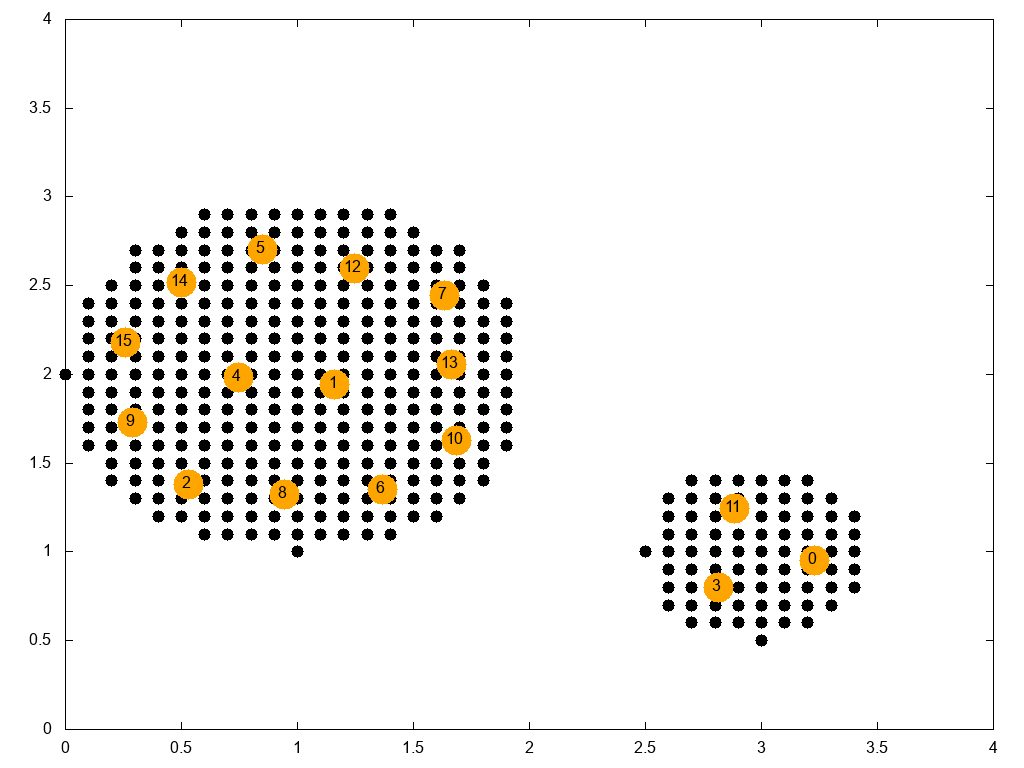
\includegraphics[scale=0.4]{netfinal.png}
\caption{Расположение нейронов после предварительного обучения ("оживления")}
\label{img:finalpos}
\end{figure}



\subsection{Вывод}

На рис. \ref{img:finalpos} видно, что в результате обучения нейроны расположились равномерно по обучающей выборке.

При предварительном обучении исходные параметры $\sigma_{min}$, $\sigma_{max}$, $\eta_{min}$, $\eta_{max}$ следует подбирать таким образом, чтобы за небольшое количество итераций "оживить все нейроны". В случае данной лабораторной работы, при установленный зачениях $\sigma_{min}$, $\sigma_{max}$, $\eta_{min}$, $\eta_{max}$ оживить все 16 нейронов удалось за 32 цикла обучения. Изменяя значения этих коэффециентов можно добиться и более хороших результатов.

В основном цикле обучения использовалась другая конфигурация весов, поэтому значения параметров $\sigma_{max} = 1.1 .. 0.6 $,  $\sigma_{min} = 0.01 .. 0.001$, $\eta_{max} = 0.6 .. 0.3$, $\eta_{min} = 0.001 .. 0.0001$ значительно меньше, по сравнению с предварительным этапом.

\subsection{Код программы}
Файл main.cpp.
\begin{verbatim}
     1	#include "NetSOM.h"
     2	#include <algorithm>
     3	#include <cmath>
     4	#include <random>
     5	
     6	void GenerateSphere(
     7	        std::vector<std::vector<double>> *points,
     8	        double x, double y, 
     9	        double r, double step)
    10	{
    11	    x = (x < 0) ? -x : x;
    12	    y = (y < 0) ? -y : y;
    13	
    14	    for (double xx = -x - r; xx <= x + r; xx += step) {
    15	        for (double yy = -y - r; yy <= y + r; yy += step) {
    16	            if (pow(xx - x, 2) + pow(yy - y, 2) <= pow(r, 2)){ 
    17	                std::vector<double> v(2);
    18	                v[0] = xx;
    19	                v[1] = yy;
    20	                points->emplace_back(std::move(v));
    21	            }
    22	        }
    23	    }
    24	}
    25	
    26	// ---------------------------------------------------------------------
------------------
    27	void SaveTrainSetToFile(std::ostream &output, const std::vector<std::vec
tor<double>> &points) {
    28	    for (size_t iPoint = 0; iPoint < points.size(); ++iPoint) {
    29	        for (size_t iCoord = 0; iCoord < points[iPoint].size(); ++iCoord
)
    30	            output << points[iPoint][iCoord] << "\t";
    31	        output << std::endl;
    32	    }
    33	}
    34	
    35	int main() {
    36	    std::vector<std::vector<double>> trainSet;
    37	    GenerateSphere (&trainSet, 1., 2., 1., 0.1);
    38	    GenerateSphere (&trainSet, 3., 1., 0.5, 0.1);
    39	    //std::random_shuffle(trainSet.begin(), trainSet.end());
    40	
    41	    Net  net;
    42	    Net::NetConfig netConf;
    43	
    44	    netConf.neurons  = 16;
    45	    netConf.inVecDim = 2;
    46	    netConf.trainEpochs = 10.;
    47	    netConf.preTrainIterations = 32;
    48	    netConf.minPotential = 0.75;
    49	    netConf.deltaMinFuncEps = 1e-3;
    50	
    51	    netConf.sigmaInitPreTrain = 2.1;
    52	    netConf.sigmaInitPreTrainMin = 0.5;
    53	    netConf.etaInitPreTrain = 1.;
    54	    netConf.etaInitPreTrainMin = 0.5;
    55	
    56	    netConf.sigmaInit = 1.;
    57	    netConf.sigmaInitMin = 1e-1;
    58	    netConf.etaInit = 0.5;
    59	    netConf.etaInitMin = 1e-3;
    60	    netConf.weightLowBound   = 0.;
    61	    netConf.weightUpperBound = 4.;
    62	
    63	    netConf.weightFileName = std::string("weight.data");
    64	
    65	    net.Init(netConf);
    66	
    67	    std::ofstream trainSetFile("train.data", std::ios::trunc);
    68	    std::ofstream weightFile(netConf.weightFileName, std::ios::trunc);
    69	    std::ofstream gnuplotFile("plot.txt", std::ios::trunc);
    70	
    71	    SaveTrainSetToFile(trainSetFile, trainSet);
    72	    //exit(1);
    73	    net.TrainGas(trainSet, weightFile);
    74	    net.CreateGnuplotAnimation(gnuplotFile);
    75	    std::cerr << "End of training " << std::endl;
    76	}

\end{verbatim}

Файл Net.cpp
\begin{verbatim}
     1	#include "Net.h"
     2	#include <iomanip>
     3	#include <random>
     4	#include <algorithm>
     5	#include <limits>
     6	#include <fstream>
     7	#include <unistd.h>
     8	
     9	void Net::Init(const NetConfig &conf) {
    10	    config = conf;
    11	    weights.resize(config.neurons * config.inVecDim);
    12	    potential.resize(config.neurons, config.minPotential);
    13	    neuronsNeighbourSequence.resize(config.neurons, 0);
    14	    victory.resize(config.neurons, 0);
    15	    RandomWeights();
    16	}
    17	bool compare(const std::pair<double, double>&i, const std::pair<double, 
double>&j){ 
    18	    return i.first < j.first; 
    19	}
    20	
    21	void Net::RandomWeights() {
    22	    std::random_device randomizer;
    23	    std::mt19937 randGen(randomizer());
    24	    std::uniform_real_distribution<> dist(config.weightLowBound, 
    25	                                          config.weightUpperBound);
    26	    double weightNorm;
    27	    double weight = 0.0;
    28	    for (size_t iNeuron = 0; iNeuron < config.neurons; ++iNeuron) {
    29	        for (size_t iWeight = 0; iWeight < config.inVecDim; ++iWeight) {
    30	            weight = dist(randGen);
    31	            std::cerr << weight << std::endl;
    32	            weights[iWeight + iNeuron * config.inVecDim] = weight;
    33	        }
    34	    }
    35	}
    36	
    37	size_t Net::DetectWinnerGas(const std::vector<double> &inVec) {
    38	
    39	    std::vector<std::pair<double, int>>  distancesToInput (config.neuron
s, std::pair<double, int> (0.0, 0));
    40	
    41	    // calculate distance for each neuron
    42	    for (size_t iNeuron = 0; iNeuron < config.neurons; ++iNeuron) {
    43	        for (size_t iWeight = 0; iWeight < config.inVecDim; ++iWeight) 
    44	            distancesToInput[iNeuron].first += pow(inVec[iWeight] - weig
hts[iWeight + iNeuron * config.inVecDim], 2);
    45	
    46	        if (potential[iNeuron] < config.minPotential)
    47	            distancesToInput[iNeuron].first = std::numeric_limits<double
>::max();
    48	        else 
    49	            distancesToInput[iNeuron].first = potential[iNeuron] * sqrt(
distancesToInput[iNeuron].first);
    50	
    51	        distancesToInput[iNeuron].second = iNeuron;
    52	    }
    53	
    54	    std::sort(distancesToInput.begin(), distancesToInput.end(), compare)
;
    55	
    56	    std::cout << "+SORTED distances" << std::endl;
    57	    for (size_t i = 0; i < distancesToInput.size(); ++i)
    58	      std::cout << distancesToInput[i].first << " " << distancesToInput[
i].second << std::endl;
    59	
    60	    std::cout << "Neightbours sequence is";
    61	    for (size_t i = 0; i < distancesToInput.size(); ++i){
    62	      neuronsNeighbourSequence[i] = distancesToInput[i].second;
    63	      std::cout << ' ' << neuronsNeighbourSequence[i];
    64	    }
    65	    std::cout << std::endl;
    66	
    67	    size_t winnerInd = distancesToInput[0].second;
    68	    std::cout << "winnerInd is " << winnerInd << std::endl;
    69	
    70	    victory[winnerInd] ++;
    71	    std::cout << "Счетчик побед: ";
    72	    for (int &a: victory)
    73	      std::cout << ' ' << a;
    74	    std::cout << '\n';
    75	
    76	    
    77	    return winnerInd;
    78	}
    79	
    80	size_t Net::GetIndexInNeuronsNeighbourSequence(size_t neuronNumber){
    81	    std::vector<int>::iterator it = std::find(neuronsNeighbourSequence.b
egin(), 
    82	                                              neuronsNeighbourSequence.e
nd(), 
    83	                                              neuronNumber);
    84	    /*if ! (it != neuronsNeighbourSequence.end())
    85	        throw std::string("Net::GetIndexInNeuronsNeighbourSequence --> E
lement Not Found!");*/
    86	
    87	    // Get index of element from iterator
    88	    int index = std::distance(neuronsNeighbourSequence.begin(), it);
    89	    return index;
    90	}
    91	
    92	void Net::AdjustWeightsKohen(size_t winnerInd, const std::vector<double>
 &inVec) {
    93	    for (size_t iNeuron = 0; iNeuron < config.neurons; ++iNeuron) {
    94	        for (size_t iWeight = 0; iWeight < config.inVecDim; ++iWeight) {
    95		          double d = fabs(iNeuron - winnerInd);
    96		          double neigbourCoeff = exp(-pow(d / sigma, 2) / 2);
    97	            weights[iWeight + iNeuron * config.inVecDim] += eta * neigbo
urCoeff 
    98	              * (inVec[iWeight] - weights[iWeight + iNeuron * config.inV
ecDim]);
    99	        }
   100	    }
   101	}
   102	
   103	void Net::AdjustWeightsGas(const std::vector<double> &inVec) {
   104	    for (size_t iNeuron = 0; iNeuron < config.neurons; ++iNeuron) {
   105	        int m = GetIndexInNeuronsNeighbourSequence(iNeuron);
   106	        double neigbourCoeff = exp(- m / sigma);
   107	        for (size_t iWeight = 0; iWeight < config.inVecDim; ++iWeight) {
   108	            weights[iWeight + iNeuron * config.inVecDim] += eta * neigbo
urCoeff 
   109	              * (inVec[iWeight] - weights[iWeight + iNeuron * config.inV
ecDim]);
   110	        }
   111	    }
   112	}
   113	
   114	void Net::AdjustPotential(size_t winnerInd) {
   115	    std::cout << std::endl << "Список потенциалов:" << 
std::endl;
   116	    for (size_t iPotential = 0; iPotential < potential.size(); iPotentia
l++) {
   117	        (iPotential == winnerInd) ? potential[iPotential] -= config.minP
otential
   118	                                  : potential[iPotential] += 1. / config
.neurons;
   119	        std::cout << potential[iPotential] << std::endl;
   120	    }
   121	    std::cout << std::endl;
   122	}
   123	
   124	void Net::TrainGas(std::vector<std::vector<double>> &trainSet,
   125	                     std::ostream &outputLabels) 
   126	{
   127	    size_t winnerInd;
   128	    double maxT;
   129	    // предварительная подготовка весов
   130	    std::random_shuffle(trainSet.begin(), trainSet.end());
   131	    PrintWeightsToFile(outputLabels, 16);
   132	
   133	    maxT = config.preTrainIterations - 1; 
   134	    for (size_t iVec = 0; iVec < config.preTrainIterations; ++iVec) {
   135	        double time = iVec + 1;  
   136	        sigma = config.sigmaInitPreTrain 
   137	              * pow(config.sigmaInitPreTrainMin / config.sigmaInitPreTra
in, time / maxT);
   138	        eta   = config.etaInitPreTrain   
   139	              * pow(config.etaInitPreTrainMin   / config.etaInitPreTrain
  , time / maxT);
   140	        winnerInd = DetectWinnerGas(trainSet[iVec]);
   141	        AdjustPotential(winnerInd);
   142	        AdjustWeightsGas(trainSet[iVec]);
   143	        PrintWeightsToFile(outputLabels, 16);
   144	    }
   145	    sleep(5);
   146	
   147	    for (int iPot = 0; iPot < potential.size(); iPot++) {
   148	        potential[iPot] = 1.;
   149	    }
   150	    maxT = config.trainEpochs * trainSet.size(); // k max = maxT, k = ti
me
   151	    double time = 0.;
   152	    for (size_t iEpoch = 0; iEpoch < config.trainEpochs; ++iEpoch) {
   153	        std::random_shuffle(trainSet.begin(), trainSet.end());
   154	        for (size_t iVec = 0; iVec < trainSet.size(); ++iVec) {
   155	            time++;
   156	            sigma = config.sigmaInit * pow(config.sigmaInitMin / config.
sigmaInit, time / maxT);
   157	            eta   = config.etaInit   * pow(config.etaInitMin   / config.
etaInit  , time / maxT);
   158	            winnerInd = DetectWinnerGas(trainSet[iVec]);
   159	            //AdjustPotential(winnerInd);
   160	            AdjustWeightsGas(trainSet[iVec]);
   161	            PrintWeightsToFile(outputLabels, 16);
   162	        }
   163	    }
   164	}
   165	
   166	void Net::PrintWeightsToFile(std::ostream &output, int precision) {
   167	    for (size_t iWeight = 0; iWeight < weights.size(); ++iWeight) {
   168	        output << std::setprecision(precision) << weights[iWeight] << "\
t";
   169	        if (iWeight % 2) {
   170	            output << iWeight / config.inVecDim << "\t";
   171	        }
   172	    }
   173	    output << std::endl << std::endl << std::endl;
   174	}
   175	
   176	void Net::CreateGnuplotAnimation(std::ofstream &stream) {
   177	    stream << " set terminal gif size 1024, 768 animate delay 0.001 loop
 -1 "<< std::endl
   178	              << " set output 'train.gif' "<< std::endl
   179	              << " set xrange [0:4] "<< std::endl
   180	              << " set yrange [0:4] "<< std::endl
   181	              << " unset key "<< std::endl              
   182	              << " stats \'" << config.weightFileName << "\' nooutput  "
<< std::endl
   183	              << " do for [i=1:int(STATS_blocks)-1] { "<< std::endl
   184	              << "     plot \"train.data\" index 0 using 1:2 pt 7 ps 2 l
c rgb \'black\',\\"<< std::endl;
   185	    for (size_t iNeuron = 0; iNeuron < config.neurons - 1; iNeuron++) {
   186	        stream << "      \"" << config.weightFileName <<"\" index(i-1) u
sing " 
   187	               <<  (iNeuron+1)*3 - 2 << ":" << (iNeuron+1)*3 - 1
   188	               << "  pt 7 ps 5 lc rgb \'orange\',\\"<< std::endl;
   189	        stream << "      \"" << config.weightFileName <<"\" index(i-1) u
sing " 
   190	               <<  (iNeuron+1)*3 - 2 << ":" << (iNeuron+1)*3 - 1 << ":" 
<< (iNeuron+1)*3
   191	               << "  with labels,\\"<< std::endl;
   192	    }
   193	    stream << "      \"" << config.weightFileName <<"\" index(i-1) using
 " 
   194	           <<  (config.neurons)*3 - 2 << ":" << (config.neurons)*3 - 1
   195	           << "  pt 7 ps 5 lc rgb \'orange\',\\"<< std::endl;
   196	    stream << "      \"" << config.weightFileName <<"\" index(i-1) using
 " 
   197	           <<  (config.neurons)*3 - 2 << ":" << (config.neurons)*3 - 1 <
< ":" << (config.neurons)*3
   198	           << "  with labels\\"<< std::endl;
   199	    stream << "}" << std::endl;
   200	
   201	    std::ofstream file;
   202	    file.open("finalpos.txt", std::ios::trunc);
   203	    file << " set terminal gif size 1024, 768 animate delay 0.001 loop -
1 "<< std::endl
   204	              << " set output 'final.gif' "<< std::endl
   205	              << " set xrange [0:4] "<< std::endl
   206	              << " set yrange [0:4] "<< std::endl
   207	              << " unset key "<< std::endl              
   208	              << " stats 'weight.data' nooutput  "<< std::endl
   209	              << " do for [i=int(STATS_blocks)-1:int(STATS_blocks)-1] { 
"<< std::endl
   210	              << "     plot \"train.data\" index 0 using 1:2 pt 7 ps 2 l
c rgb \'black\',\\"<< std::endl;
   211	    for (size_t iNeuron = 0; iNeuron < config.neurons - 1; iNeuron++) {
   212	        file << "      \"" << config.weightFileName <<"\" index(i-1) usi
ng " 
   213	               <<  (iNeuron+1)*3 - 2 << ":" << (iNeuron+1)*3 - 1
   214	               << "  pt 7 ps 5 lc rgb \'orange\',\\"<< std::endl;
   215	        file << "      \"" << config.weightFileName <<"\" index(i-1) usi
ng " 
   216	               <<  (iNeuron+1)*3 - 2 << ":" << (iNeuron+1)*3 - 1 << ":" 
<< (iNeuron+1)*3
   217	               << "  with labels,\\"<< std::endl;
   218	    }
   219	    file << "      \"" << config.weightFileName <<"\" index(i-1) using "
 
   220	           <<  (config.neurons)*3 - 2 << ":" << (config.neurons)*3 - 1
   221	           << "  pt 7 ps 5 lc rgb \'orange\',\\"<< std::endl;
   222	    file << "      \"" << config.weightFileName <<"\" index(i-1) using "
 
   223	           <<  (config.neurons)*3 - 2 << ":" << (config.neurons)*3 - 1 <
< ":" << (config.neurons)*3
   224	           << "  with labels\\"<< std::endl;
   225	    file << "}" << std::endl;
   226	
   227	    std::ofstream fileStart;
   228	    fileStart.open("startpos.txt", std::ios::trunc);
   229	    fileStart << " set terminal gif size 1024, 768 animate delay 0.001 l
oop -1 "<< std::endl
   230	              << " set output 'startpos.gif' "<< std::endl
   231	              << " set xrange [0:4] "<< std::endl
   232	              << " set yrange [0:4] "<< std::endl
   233	              << " unset key "<< std::endl              
   234	              << " stats 'weight.data' nooutput  "<< std::endl
   235	              << " do for [i=1:1] { "<< std::endl
   236	              << "     plot \"train.data\" index 0 using 1:2 pt 7 ps 2 l
c rgb \'black\',\\"<< std::endl;
   237	    for (size_t iNeuron = 0; iNeuron < config.neurons - 1; iNeuron++) {
   238	        fileStart << "      \"" << config.weightFileName <<"\" index(i-1
) using " 
   239	               <<  (iNeuron+1)*3 - 2 << ":" << (iNeuron+1)*3 - 1
   240	               << "  pt 7 ps 5 lc rgb \'orange\',\\"<< std::endl;
   241	        fileStart << "      \"" << config.weightFileName <<"\" index(i-1
) using " 
   242	               <<  (iNeuron+1)*3 - 2 << ":" << (iNeuron+1)*3 - 1 << ":" 
<< (iNeuron+1)*3
   243	               << "  with labels,\\"<< std::endl;
   244	    }
   245	    fileStart << "      \"" << config.weightFileName <<"\" index(i-1) us
ing " 
   246	           <<  (config.neurons)*3 - 2 << ":" << (config.neurons)*3 - 1
   247	           << "  pt 7 ps 5 lc rgb \'orange\',\\"<< std::endl;
   248	    fileStart << "      \"" << config.weightFileName <<"\" index(i-1) us
ing " 
   249	           <<  (config.neurons)*3 - 2 << ":" << (config.neurons)*3 - 1 <
< ":" << (config.neurons)*3
   250	           << "  with labels\\"<< std::endl;
   251	    fileStart << "}" << std::endl;
   252	
   253	    std::ofstream filePreTrain;
   254	    filePreTrain.open("afterPreTrain.txt", std::ios::trunc);
   255	    int outIter = config.preTrainIterations;
   256	    filePreTrain << " set terminal gif size 1024, 768 animate delay 0.00
1 loop -1 "<< std::endl
   257	              << " set output 'afterPreTrain.gif' "<< std::endl
   258	              << " set xrange [0:4] "<< std::endl
   259	              << " set yrange [0:4] "<< std::endl
   260	              << " unset key "<< std::endl              
   261	              << " stats 'weight.data' nooutput  "<< std::endl
   262	              << " do for [i=" << outIter << ":" << outIter <<"] { "<< s
td::endl
   263	              << "     plot \"train.data\" index 0 using 1:2 pt 7 ps 2 l
c rgb \'black\',\\"<< std::endl;
   264	    for (size_t iNeuron = 0; iNeuron < config.neurons - 1; iNeuron++) {
   265	        filePreTrain << "      \"" << config.weightFileName <<"\" index(
i-1) using " 
   266	               <<  (iNeuron+1)*3 - 2 << ":" << (iNeuron+1)*3 - 1
   267	               << "  pt 7 ps 5 lc rgb \'orange\',\\"<< std::endl;
   268	        filePreTrain << "      \"" << config.weightFileName <<"\" index(
i-1) using " 
   269	               <<  (iNeuron+1)*3 - 2 << ":" << (iNeuron+1)*3 - 1 << ":" 
<< (iNeuron+1)*3
   270	               << "  with labels,\\"<< std::endl;
   271	    }
   272	    filePreTrain << "      \"" << config.weightFileName <<"\" index(i-1)
 using " 
   273	           <<  (config.neurons)*3 - 2 << ":" << (config.neurons)*3 - 1
   274	           << "  pt 7 ps 5 lc rgb \'orange\',\\"<< std::endl;
   275	    filePreTrain << "      \"" << config.weightFileName <<"\" index(i-1)
 using " 
   276	           <<  (config.neurons)*3 - 2 << ":" << (config.neurons)*3 - 1 <
< ":" << (config.neurons)*3
   277	           << "  with labels\\"<< std::endl;
   278	    filePreTrain << "}" << std::endl;
   279	
   280	}
\end{verbatim}

Файл Net.h
\begin{verbatim}
     1	#include <vector>
     2	#include <iostream>
     3	#include <fstream>
     4	using size_t = std::size_t;
     5	
     6	class Net {
     7	public:
     8	    struct NetConfig {
     9	        size_t neurons;
    10	        size_t inVecDim;
    11	        int    trainEpochs;
    12	        int    preTrainIterations;
    13	        double minPotential;
    14	        double deltaMinFuncEps;
    15	        
    16	        double sigmaInitPreTrain;
    17	        double etaInitPreTrain;
    18	        double sigmaInitPreTrainMin;
    19	        double etaInitPreTrainMin;
    20	        
    21	        double sigmaInit;
    22	        double etaInit;
    23	        double sigmaInitMin;
    24	        double etaInitMin;
    25	
    26	        double weightLowBound;
    27	        double weightUpperBound;
    28	
    29	        std::string weightFileName;
    30	    };
    31	
    32	    void Init(const NetConfig &conf);
    33	    void TrainKohen(std::vector<std::vector<double>> &trainSet, std::ost
ream &outputLabels);
    34	    void TrainGas(std::vector<std::vector<double>> &trainSet, std::ostre
am &outputLabels);
    35	    void PrintWeightsToFile(std::ostream &output, int precision);
    36	    void CreateGnuplotAnimation(std::ofstream &stream);
    37	    size_t DetectWinnerKohen(const std::vector<double> &inVec);
    38	    size_t DetectWinnerGas(const std::vector<double> &inVec);
    39	
    40	private:
    41	    NetConfig config;
    42	    std::vector<double>   weights;
    43	    std::vector<double>   potential;
    44	    std::vector<int>      neuronsNeighbourSequence; // for DetectWinnerK
ohen
    45	    std::vector<int>      victory;
    46	    double sigma;
    47	    double eta;
    48	    void RandomWeights();
    49	    void AdjustWeightsKohen(size_t winnerInd, const std::vector<double> 
&inVec);
    50	    void AdjustWeightsGas(const std::vector<double> &inVec);
    51	    void AdjustPotential(size_t winnerInd);
    52	    void AdjustPotentialInverted(size_t winnerInd);
    53	    size_t GetIndexInNeuronsNeighbourSequence(size_t neuronNumber);
    54	};

\end{verbatim}
